% =========================================================================== %
% Yes. This is a document.

\documentclass[
	english,
	aspectratio=169,
	table
]{beamer}

% =========================================================================== %
% Theme
\usepackage{scrlfile}
	\ReplacePackage{beamerthemeSHUR}{./sty/beamerthemeSHUR}
	\ReplacePackage{beamerinnerthemefancy}{./sty/beamerinnerthemefancy}
	\ReplacePackage{beamerouterthemedecolines}{./sty/beamerouterthemedecolines}
	\ReplacePackage{beamercolorthemechameleon}{./sty/beamercolorthemechameleon}

\usetheme[
	pageofpages=/,
	bullet=circle,
	titleline=true,
	alternativetitlepage=true,
	watermark="",
	watermarkheight=0px,
	watermarkheightmult=0
	]
{SHUR}

% =========================================================================== %
% the usual stuff

\usepackage[utf8]{inputenc}
\usepackage[T1]{fontenc}
\usepackage{babel}
\usepackage{lmodern}
\usepackage{microtype}
\usepackage{csquotes}
\usepackage{xspace}

\usepackage{tabularx}
\usepackage{booktabs}
\usepackage{multirow}

\usepackage{color, colortbl}
\usepackage{xcolor}
	\definecolor{tabhighlight}{RGB}{230,240,255}

\usepackage{tabto}

\usepackage{minted}
	\usemintedstyle{friendly}

\usepackage{tikz}
	\usetikzlibrary{positioning}
	\usetikzlibrary{matrix}
	\usetikzlibrary{shapes.geometric}
	\usetikzlibrary{backgrounds}
	\usetikzlibrary{calc}
	\usetikzlibrary{decorations.pathreplacing}
	\tikzstyle{every picture}+=[remember picture] 
\usepackage{adjustbox}

\usepackage{amsmath}
\usepackage{physics}

\usepackage[most]{tcolorbox}
	\tcbsetforeverylayer
		{colback=cyan!10!white,
		 colframe=cyan!75!black,
		 arc=0pt,
		 outer arc=0pt
		}
	\newtcolorbox{codebox}[1][Code]
		{colback=black!5!white,
		 colframe=blue!40!black,
		 title=#1,
		 leftupper=6mm
		}
	\newtcolorbox{cmdbox}[1][Command Line]
		{colback=black,
		 coltext=white,
		 fontupper=\ttfamily ,
		 colframe=blue!40!black,
		 title=#1,
		 outer arc=0pt
		}
	\newtcolorbox{warnbox}[1][Warning]
		{colback=black!5!white,
		 colframe=red!40!black,
		 title=#1
		}
	\newtcolorbox{hintbox}[1][Hint]
		{colback=black!5!white,
		 colframe=green!40!black,
		 title=#1
		}
	\newtcolorbox{defbox}[1][Code]
		{colback=cyan!10!white,
		 colframe=cyan!90!black,
		 title=#1
		}
%==============================================================================%
% GLOBAL MACROS

\newcommand*{\zB}{e.\,g. }
\newcommand*{\ie}{i.\,e. }

\newcommand{\Thus}{\ensuremath{\Rightarrow}\xspace}
\newcommand{\thus}{\ensuremath{\rightarrow}\xspace}

\newcommand*{\tabcrlf}{\\ \midrule}			% actually still allows for optional argument

\newcommand*{\inPy}[1]{\mintinline{python}{#1}}

\newcommand*{\todo}[1]{{\color{red}TODO: #1}}

% =========================================================================== %

\author{Stefan Hartinger}
\title{Python for Scientists}
\subtitle{Part 3: Integration and Derivation with Numpy and SciPy}
\institute{Department of Just Some Dude Who Likes to Talk}
\date{Spring 2023}

% =========================================================================== %

\begin{document}
% =========================================================================== %

\begin{frame}[t,plain]
\titlepage
\end{frame}

% =========================================================================== %

\begin{frame}{Integration vs. Differentiation}
%
\begin{columns}
\column{.6\linewidth}
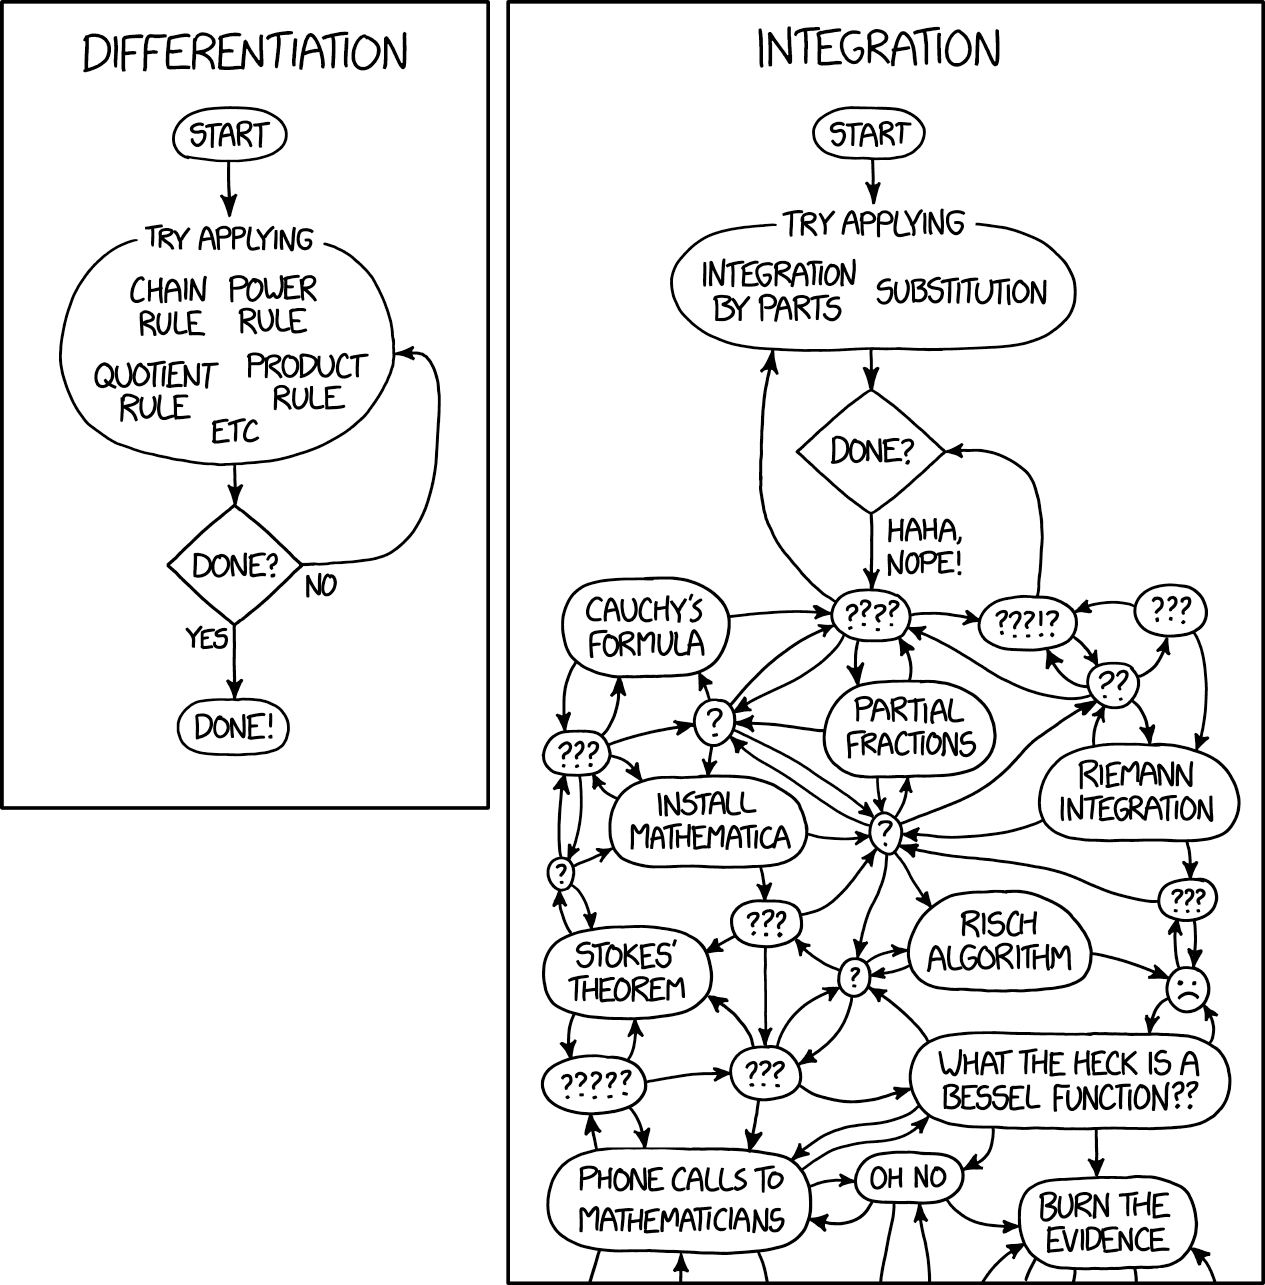
\includegraphics[width=0.8\linewidth]{./gfx/03-xkcd-differentiation_and_integration}\\
%
\column{.3\linewidth}
\scriptsize
	\emph{\enquote{Symbolic integration} is when you theatrically go through the motions of finding integrals, 
		but the actual result you get doesn't matter because it's purely symbolic.}

	\vspace{6pt}
	\url{https://xkcd.com/2117/}
\end{columns}
%
\end{frame}

% =========================================================================== %

\begin{frame}{Scope for Today}
%
\begin{itemize}
\item Numerical Derivatives
	\begin{itemize}
	\item Central difference method
	\item \texttt{numpy.gradient}
	\item Laplace operator by convolution
	\end{itemize}
\item Integrals
	\begin{itemize}
	\item Ideas for approximations
	\item SciPy to the rescue
	\end{itemize}
\item Next Time: Differential Equations
	\begin{itemize}
	\item By Integration and by eigenvalue
	\item First order, Second and higher order
	\item Partial differential equations
	\end{itemize}
\end{itemize}
%
\end{frame}

% =========================================================================== %

\begin{frame}%{Derivatives}
%
\begin{defbox}[Definitions of Derivative]
\begin{align}
	\dv{x} f(x)
&=
	\lim_{\varepsilon \to 0}
		\dfrac{f(x + \varepsilon) - f(x)}{\varepsilon}
\\
	\dv{x} f(x)
&=
	\lim_{\varepsilon \to 0}
		\dfrac{f(x + \varepsilon) - f(x - \varepsilon)}{2\varepsilon}
\end{align}
\end{defbox}
%
\begin{itemize}
\item Standard approach (1): Finite Differences: Set $\varepsilon$ to an arbitrary small but nonzero value
\item Works, but error-prone
	\begin{itemize}
	\item Essentially amplified rounding errors
	\item Next Slides
	\end{itemize}
\item Small mitigation: central difference method (2)
	\begin{itemize}
	\item Better, but does not get rid of the underlying problem
	\end{itemize}
\end{itemize}
%
\end{frame}

% =========================================================================== %

\begin{frame}{Why The Central Difference Approximation Is More Accurate}
%
\begin{flalign}
\text{Taylor Expansion} \quad
&
	f(x + \varepsilon) 
~\approx~
	f(x) + f'(x) \varepsilon {\color{gray} + \dfrac{1}{2} f''(x) \varepsilon^2 + f'''(x) \varepsilon^3}
\\
\text{Implies} \quad
&
\dfrac
	{f(x + \varepsilon) - f(x)}
	{\varepsilon}
~\approx~
	f'(x) + 
	{\color{blue} \underbrace{\dfrac{1}{2} f''(x) \varepsilon}_{\mathcal{O}(\varepsilon)}} +
	{\color{gray} \dfrac{1}{6} f'''(x) \varepsilon^2}
	\label{eqn:forward-difference}
\\
\text{Likewise} \quad
&
	f(x - \varepsilon) 
~\approx~
	f(x) - f'(x) \varepsilon + {\color{gray} \dfrac{1}{2} f''(x) \varepsilon^2 - f'''(x) \varepsilon^3}
\\
\text{Implies} \quad
&
	\dfrac
		{f(x - \varepsilon) - f(x)}
		{\varepsilon}
~\approx~
	-f'(x) 
	{\color{blue}+\dfrac{1}{2} f''(x) \varepsilon}
	{\color{gray}
	 -\dfrac{1}{6} f'''(x) \varepsilon^2
	}\label{eqn:backward-difference}
\\
\text{Subtract (\ref{eqn:backward-difference}) from (\ref{eqn:forward-difference}) to get} \quad
&
\dfrac
	{f(x + \varepsilon) - f(x - \varepsilon)}
	{2\varepsilon}
~\approx~
	f'(x) 
	{\color{blue} + 0\varepsilon}
	{\color{purple} + \underbrace{
		\dfrac{1}{12} f'''(x) \varepsilon^2
	}_{\mathcal{O}(\varepsilon^2)}}
\end{flalign}
%
\end{frame}

% =========================================================================== %

\begin{frame}{Why This Won't Save Our Asses}
%
\begin{itemize}
\item IEEE 754: Standard for Floating-Point Arithmetic
	\begin{itemize}
	\item Institute of Electrical and Electronics Engineers (IEEE)
	\item Remember: only two symbols: 1 and 0. In particular, no comma
	\item Split bits in three parts: sign, mantissa, exponent
	\item Essentially: scientific notation: $0.0527 = 5.27 \cdot 10^{-2}$
	\item Mantissa: limited number of bits $\rightsquigarrow$ limited number of digits
	\item Rounding error when subtracting similar values
	\item Amplified when dividing by a small number
	\end{itemize}
\item No real way around this.
	\begin{itemize}
	\item Always bad approximations for highly oscillatory functions
	\item Doesn't mean always bad
	\item But keep in mind to take derivatives with a grain of salt
	\end{itemize}
\item In particular bad for \emph{too small} values of $\varepsilon$.
	\begin{itemize}
	\item Python's \inPy{float} type allows ca. 15 significant digits
	\item $\varepsilon \approx 10^{-6}$ usually a good choice; smaller for \emph{very fast} oscillations
	\end{itemize}
\end{itemize}
%
\end{frame}

% =========================================================================== %

\begin{frame}{Exampe in Numbers}
%
\begin{itemize}
\item Assume: 5 significant digits
\item Mathematical precision shown in gray
\item \texttt{f(x) = 12.345{\color{gray}1234}}
\item \texttt{f(x + $\varepsilon$) = 12.354{\color{gray}3210}}
\item \texttt{f(x + $\varepsilon$) - f(x) = 0.009{\color{gray}1976}}
\item \texttt{$\varepsilon$ = 0.001 = 10}$^{-3}$
\item Result with mathematical precision: \texttt{9.1976}
\item Result due to rounding errors: \texttt{9.00000}
\item[\Thus] Off by 2.1\%
\item[\Thus] Errors propagate and accumulate
\end{itemize}
%
\end{frame}

% =========================================================================== %

\begin{frame}[fragile]{In Practice}
%
\begin{columns}
\column{.4\linewidth}
\begin{itemize}
\item Comparing derivative methods for $f(x) = \sin(\dfrac{1}{x^2 + c})$ with $c = 0.02$
	\begin{itemize}
	\item Ever faster oscillations closer to 0
	\item Control oscillation via $c$; smaller means faster
	\item Code for subsequent figures on GRIPS
	\end{itemize}
\end{itemize}
%
\column{.4\linewidth}
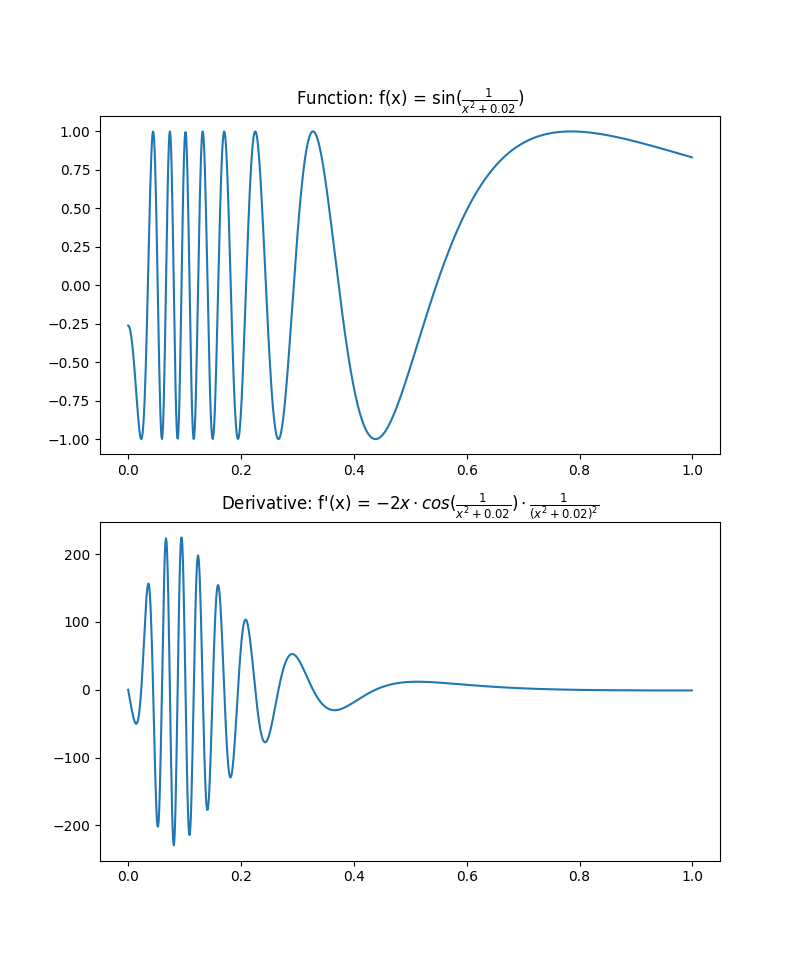
\includegraphics[width=\linewidth]{./gfx/03-derivative-functions}
\end{columns}
%
\end{frame}

% =========================================================================== %

\begin{frame}{Comparing Methods}
%
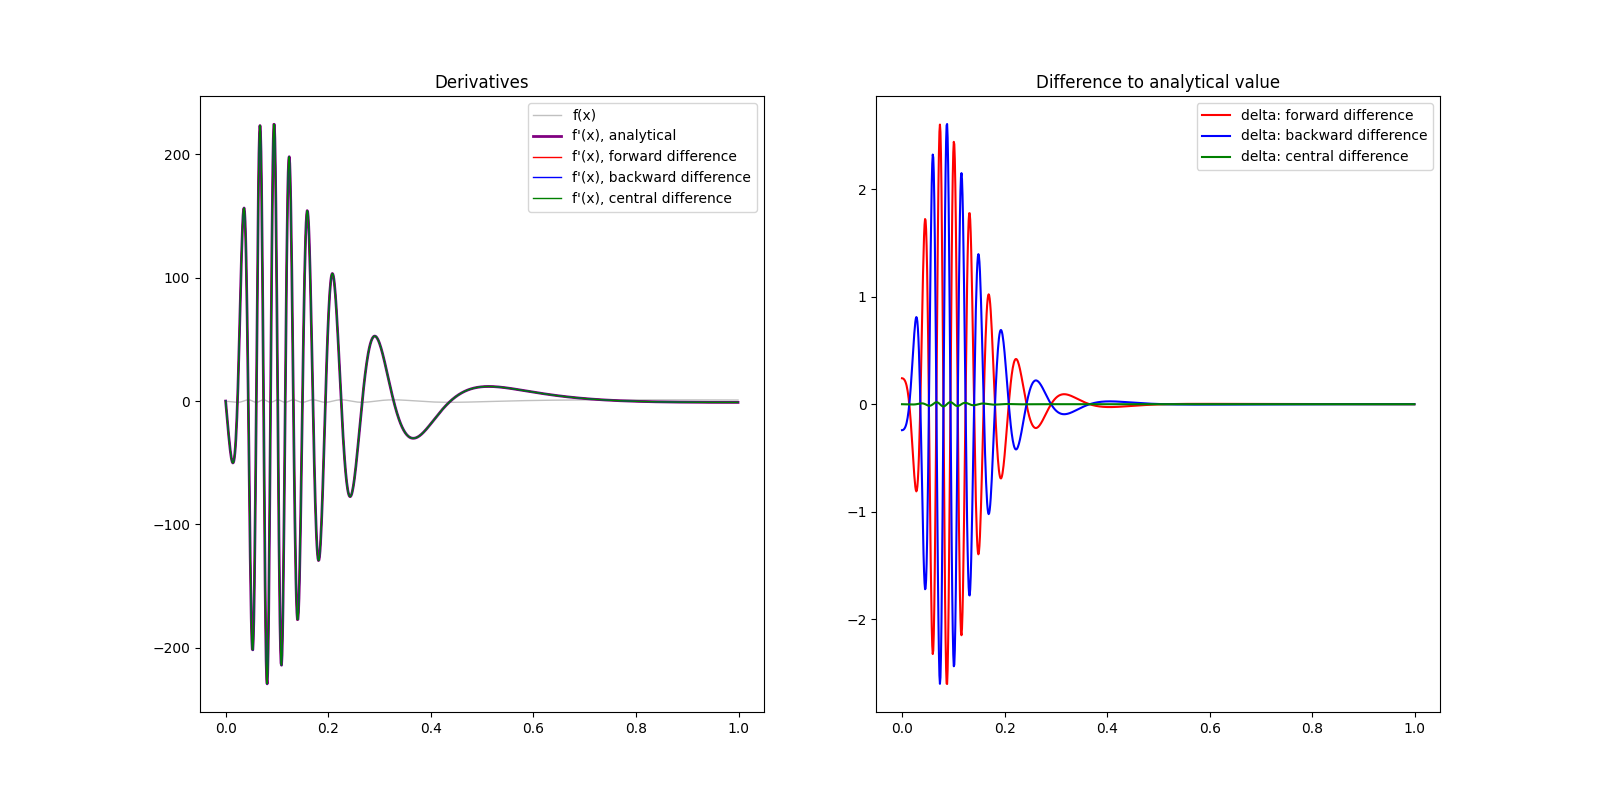
\includegraphics[width=\linewidth]{./gfx/03-derivative-methods}
%
\end{frame}

% =========================================================================== %

\begin{frame}{Comparing Epsilons (Central Difference Method)}
%
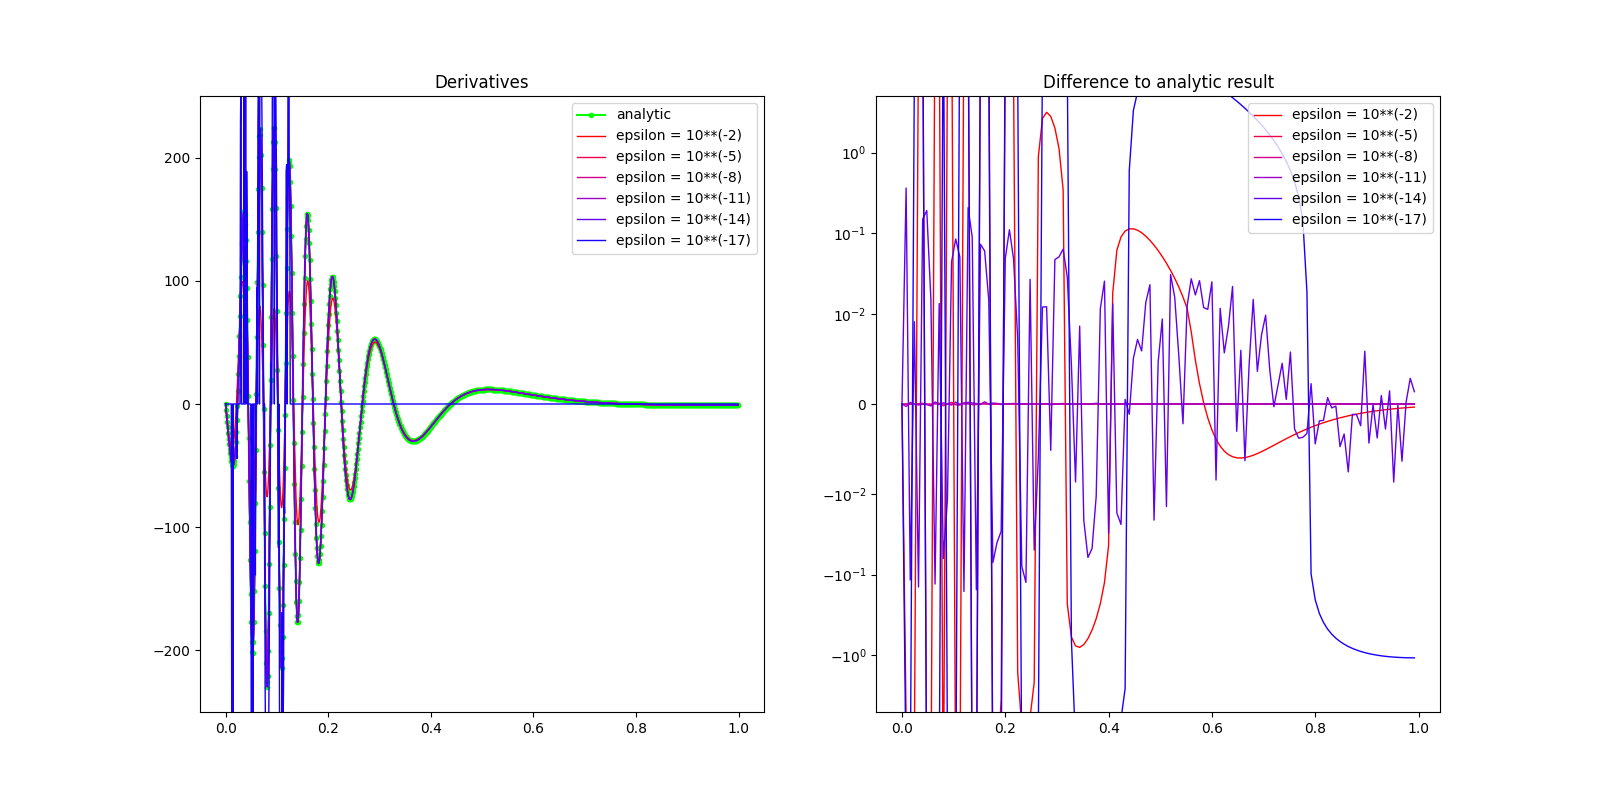
\includegraphics[width=\linewidth]{./gfx/03-derivative-epsilons}
%
\end{frame}

% =========================================================================== %

\begin{frame}{In Practice: Numbers}
%
\begin{itemize}
\item Forward/Backward difference vs. central difference
	\begin{itemize}
	\item Maximum error forward/backward difference: ca. 1.13\%
	\item Maximum error central difference: ca. 0.0088\%
	\end{itemize}
\item Effect of Epsilon
	\vspace{-6pt}
	\begin{columns}[T]
		\column{.4\linewidth}
		\begin{itemize}
		\item $10^{-2}: 1028.2\%$
		\item $10^{-3}: 12.8\%$
		\item $10^{-4}: 0.128\%$
		\item $10^{-5} ... 10^{-8}: < 0.001\%$
		\end{itemize}
		\column{.4\linewidth}
		\begin{itemize}
		\item $10^{-9}: 0.002\%$
		\item $10^{-12}: 0.143\%$
		\item $10^{-13}: 11.9\%$
		\item $10^{-15}: 100.0\%$
		\end{itemize}
	\end{columns}
	\vspace{6pt}
	
\item Numbers are specific for this scenario -- vary parameter \texttt{c} and get totally different results
\item Order of magnitude is something we can draw from this example, though
\item Epsilon should be at least an order smaller than the \enquote{wavelength/period} of the oscillation
\end{itemize}
%
\end{frame}

% =========================================================================== %

\begin{frame}{Computing Derivatives with Numpy}
%
\begin{itemize}
\item Numpy to the rescue: central difference method implemented well and fast
\item Pre-compute $f(x)$ for a number of $x_i$: $f_i = f(x_i)$
\item $\varepsilon_i = x_i - x_{i - 1}$ \Thus Variable resolution possible
	\begin{itemize}
	\item My default pattern, though:\\
		\texttt{X = np.arange(start, stop, epsilon)}\\
		\texttt{Y = f(X)}
	\end{itemize}
\item Get the derivative via\\
	\texttt{Y\_prime = np.gradient(Y, X)}\\
	or via\\
	\texttt{Y\_prime = np.gradient(Y, epsilon)}
\item Actually, passing \texttt{X} is optional; assume index is x-coordinate if omitted
\end{itemize}
%
\end{frame}

% =========================================================================== %

\begin{frame}{Numpy Goodies: Multidimensional Derivatives}
%
\begin{itemize}
\item Scalar Fields
	\begin{itemize}
	\item Just pass a multidimensional array as first parameter
	\item To get derivative along one axis:\\
		\texttt{dF\_wrt\_axis\_i = np.gradient(field, coordinates, axis=i)}\\
		or\\
		\texttt{dF\_wrt\_axis\_i = np.gradient(field, epsilon, axis=i)}\\
	\item To get derivative along \emph{all} axes:\\
		\texttt{list\_of\_derivatives = np.gradient(field, epsilon)}
	\end{itemize}
\item Vector Fields ...
	\begin{itemize}
	\item ... are just multiple scalar fields
	\item \enquote{simply} select the correct axis
	\end{itemize}
\end{itemize}
%
\end{frame}

% =========================================================================== %

\begin{frame}[fragile]
%
\begin{codebox}[Scalar Field and Derivatives]
\begin{minted}[linenos, fontsize=\scriptsize]{python3}
import matplotlib.pyplot as plt
import numpy as np

epsilon = 0.05
rng = np.arange(-1.0, 1.0 + epsilon, epsilon)
X, Y = np.meshgrid(rng, rng, indexing='ij')
R = np.sqrt(X ** 2 + Y ** 2)
F = np.exp(-R) * np.cos(10 * R)

dFx, dFy = np.gradient(F, epsilon)

fig, axs = plt.subplots(1, 2)
fig.set_size_inches(16, 8)

axs[0].set_title("f(x, y)")
axs[0].pcolor(X, Y, F)

axs[1].set_title("grad f(x, y)")
axs[1].quiver(X, Y, dFx, dFy)

plt.show()
\end{minted}
\end{codebox}
%
\end{frame}

% =========================================================================== %\\

\begin{frame}
%
\begin{defbox}[Output: Scalar field and derivatives]
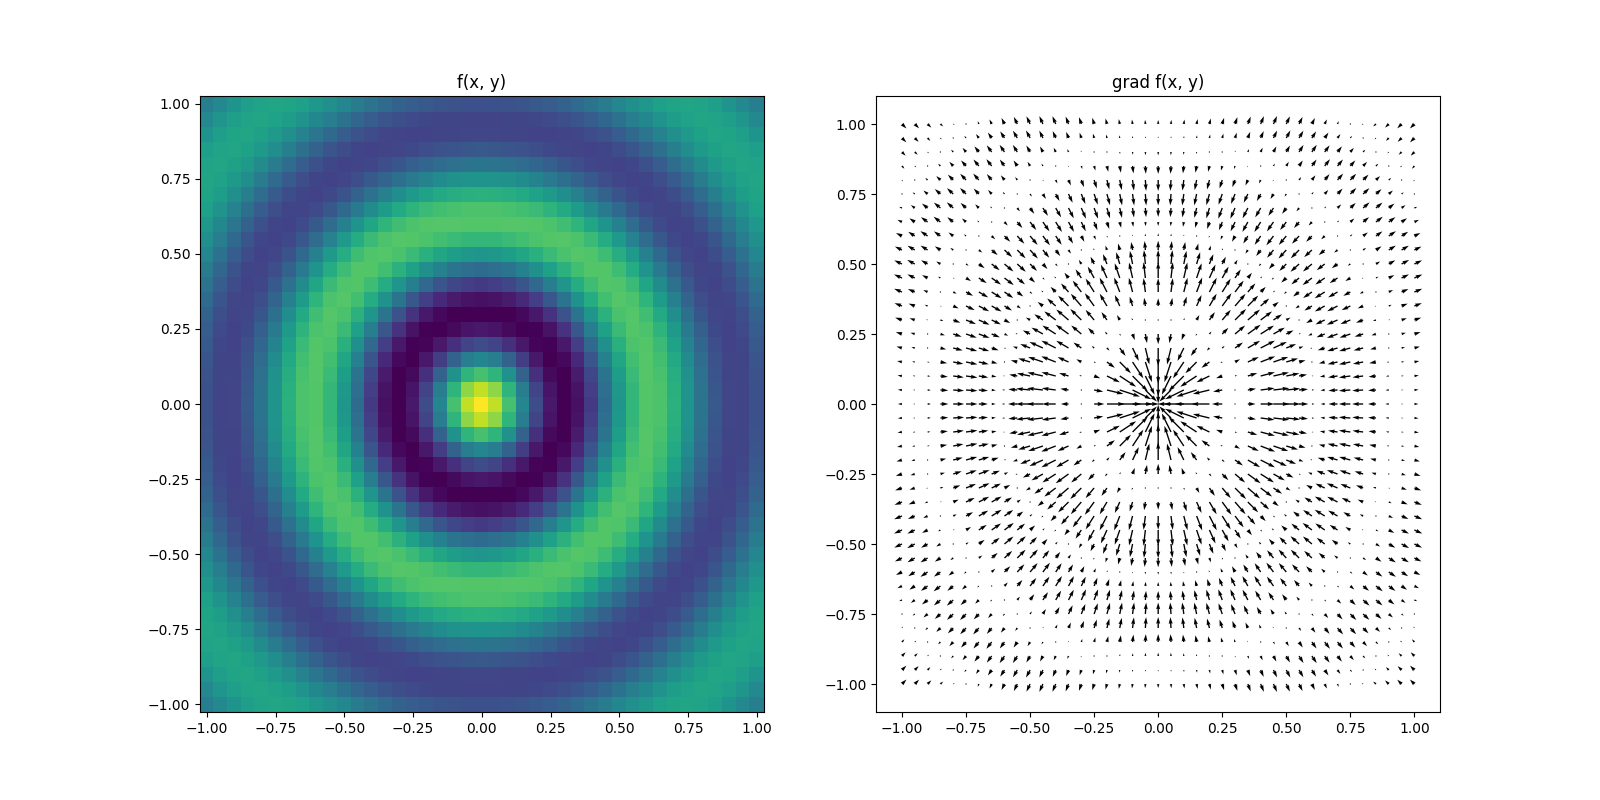
\includegraphics[width=\linewidth]{./gfx/03-derivatives-numpy}
\end{defbox}
%
\end{frame}


% =========================================================================== %

\begin{frame}
%
\begin{defbox}[Convolutions]
\vspace{-9pt}
\begin{flalign}
\text{Continuous Definition} &&
	(f \ast g)(t) 
&=
	\int_{-\infty}^{\infty} f(t - \tau) g(t) \dd{\tau}
\\
\text{Discrete Definition} &&
	(\vec{f} \ast \vec{g})_i
&=
	\sum_{j=1}^{\dim(\vec{g})}
		f_{(i-j)} \; g_j
\end{flalign}
%
\begin{columns}[T]
\column{.4\linewidth}
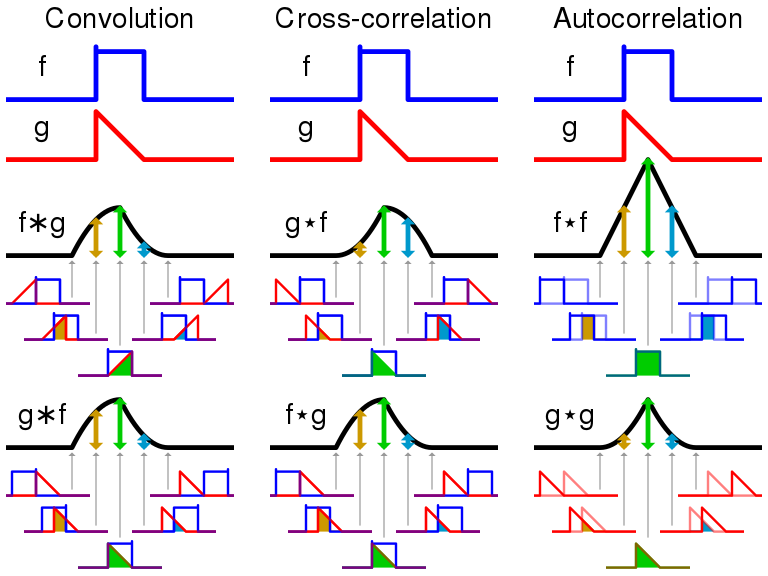
\includegraphics[width=\linewidth]{./gfx/03-convolution}
%
\column{.5\linewidth}
\begin{itemize}
\item Idea: move a \enquote{weight window function} over $f$ and collect contributions
\item Discrete form: $f_{(i-j)} = 0$ for $i - j < 1$
\item Picture: Wikipedia User Cmglee\\
	\url{https://en.wikipedia.org/wiki/File:Comparison_convolution_correlation.svg}
\end{itemize}
\end{columns}
\end{defbox}
%
\end{frame}

% =========================================================================== %

\begin{frame}{Derivatives as Convolutions}
%
\begin{columns}
\column{.25\linewidth}
\small
\begin{align*}
	\dv{f}{x}% f(x)
&\approx
	\dfrac
		{f(x + \varepsilon) - f(x - \varepsilon)}
		{2\varepsilon}
	\\
&\to
	\dfrac
		{f_{i+1} - f_{i-1}}
		{2\varepsilon}
	\\
&\to
	\vec{f} \ast {}^{1}/_{2\varepsilon}
	\begin{pmatrix}
	-1 & 0 & 1
	\end{pmatrix}
\\
	\dv[2]{f}{x}
&\approx
	\dfrac
		{f(x - \varepsilon) -2 f(x) + f(x + \varepsilon)}
		{\varepsilon^2}
	\\
&\to
	\dfrac
		{f_{i-1} - 2 f_i + f_{i+1}}
		{\varepsilon^2}
	\\
&\to
	\vec{f} \ast {}^{1}/_{\varepsilon^2}
	\begin{pmatrix}
	1 & -2 & 1
	\end{pmatrix}
\end{align*}
%
\column{.56\linewidth}
\begin{defbox}[2$^{nd}$ Derivative -- Proof, leftupper=1mm]
\scriptsize
\begin{align*}
f(x + \varepsilon) &\approx
	f(x) + f'(x)\varepsilon + \dfrac{1}{2}f''(x)\varepsilon^2 + \dfrac{1}{6}f'''(x)\varepsilon^3 + \mathcal{O}(\varepsilon^4)
\\
f(x - \varepsilon) &\approx
	f(x) - f'(x)\varepsilon + \dfrac{1}{2}f''(x)\varepsilon^2 - \dfrac{1}{6}f'''(x)\varepsilon^3 + \mathcal{O}(\varepsilon^4)
\end{align*}
Add these together to get
\begin{align*}
f''(x) &\approx
	\dfrac
		{f(x - \varepsilon) - 2f(x) + f(x + \varepsilon)}
		{\varepsilon^2}
	+ \mathcal{O}(\varepsilon^2)
\end{align*}
\end{defbox}
\end{columns}
%
\end{frame}

% =========================================================================== %

\begin{frame}{Laplacian as Convolution Kernel}
%
\begin{itemize}
\item Generalize Convolution in $N$ dimensions: get \enquote{rotated} (transposed) convolution kernels
\item $\pdv{y} \to \begin{pmatrix}
-1 \\ 0 \\ +1
\end{pmatrix}$ with $f(x, y) \to f_{y,x}$
\item 2D Laplacian:
$
\laplacian_{\text{2D}} = \pdv[2]{x} + \pdv[2]{y}
\to \begin{pmatrix}
  0 & +1 &  0 \\
 +1 & -4 & +1 \\
  0 & +1 &  0 
\end{pmatrix}
$
\end{itemize}
%
\begin{hintbox}[Higher Order Derivatives]
\small
You can get higher order derivatives by recursively applying the formulae for the 1$^{st}$ and 2$^{nd}$ derivative. E.\;g.
$\dv[3]{x} \to
{}^{1}/_{4\varepsilon^3}
\begin{pmatrix}
+1 & -2 & 0 & +2 & -1
\end{pmatrix}$
\end{hintbox}
%
\end{frame}

% =========================================================================== %

\begin{frame}{Convolution in Code: \texttt{scipy.signal.convolve}}
%
\begin{itemize}
\item All of this ready to use in \texttt{scipy.signal.convolve}
\item Simply define kernel as numpy ndarray
\item \texttt{result = convolve(data, kernel)}
\item Optional parameter \texttt{mode}
	\begin{itemize}
	\item String, controls padding
	\item Default: \texttt{full} add extra null columns/rows/layers/... at the right/lower/... end to get \texttt{result.shape == data.shape}
	\item \texttt{valid}: No padding; \texttt{result} will have less rows/columns
	\item \texttt{same}: add extra nulls symmetrically to get \texttt{result.shape == data.shape} with padding surrounding the regular data (most useful for derivatives)
	\end{itemize}
\end{itemize}
%
\end{frame}

% =========================================================================== %

\begin{frame}[fragile]
%
\begin{codebox}[Second Derivative By Convolution]
\begin{minted}[linenos, fontsize=\scriptsize]{python3}
import numpy as np
from scipy.signal import convolve

data = np.arange(10)**2    # "f(x) = x**2"
kernel = np.array([1, -2, 1])

derivative2 = convolve(data, kernel, mode='same')
print(derivative2)
\end{minted}
\end{codebox}
%
\begin{cmdbox}[Output: Second Derivative By Convolution]
\begin{minted}[fontsize=\scriptsize]{text}
[  1   2   2   2   2   2   2   2   2 -98]
\end{minted}
\end{cmdbox}
%
\begin{hintbox}[Derivatives on open intervals]
\small
Remember how the derivative is only defined on open intervals? As direct consequence, this discrete derivative is ill defined on the boundaries.
\end{hintbox}
%
\end{frame}

% =========================================================================== %

\begin{frame}[fragile]{Numerical Integrals}
%
\begin{itemize}
\item Comparatively simple
\item Variations of: sum up $\Delta f \cdot \varepsilon$
	\begin{itemize}
	\item Some smart ideas to get a better $\Delta{f}$ from the integrand
	\item Some smart ideas to save time
	\end{itemize}
\item Floating point accuracy less of a problem
	\begin{itemize}
	\item \emph{Multiplying} by $\varepsilon$ instead of dividing
	\item No amplification of rounding errors
	\end{itemize}
\end{itemize}
%
\begin{hintbox}[Quadrature]
An the subsequent slides, the word \emph{quadrature} will appear frequently. It simply means \emph{numerical approximation to an integral}.
\end{hintbox}
%
\end{frame}

% =========================================================================== %

\begin{frame}{Newton-Cotes, Simpson, Boole}
%
\begin{minipage}{.6\linewidth}
\small
\begin{itemize}
\item Naively: rectangle rule: $\Delta f$ = integrand. Evaluate and sum up $f(x) \cdot \varepsilon$ in $x_i = x_0 + i \cdot \varepsilon$.
	\vspace{-4pt}
	\begin{itemize}
	\item Accuracy $\propto \varepsilon f'(x)$ 
	\end{itemize}
	\vspace{-9pt}
\item First improvement: trapezoid rule: use $\Delta f = \dfrac{f(x) + f(x + \varepsilon)}{2}$
	\vspace{-4pt}
	\begin{itemize}
	\item Accuracy $\propto \varepsilon^3 f''(x)$ 
	\end{itemize}
	\vspace{-4pt}
\item Second improvement: Simpson's rule: approximate function between $f(x)$ and $f(x + \varepsilon)$ as parabola
	\begin{itemize}
	\item Exact integral for polynomials is known
	\item $\Delta f = \dfrac{f(x) + 4f(x + \varepsilon) + f(x + 2\varepsilon)}{3}$
	\item Accuracy $\propto \varepsilon^5 f^{(4)}(x)$ 
	\end{itemize}
	\vspace{-6pt}
\item Boole's rule: same ideas for 4$^{th}$ order polynomials
	\begin{itemize}
	\item Accuracy $\propto \varepsilon^7 f^{(6)}(x)$ 
	\end{itemize}
\end{itemize}
\end{minipage}
%
\begin{minipage}{.39\linewidth}
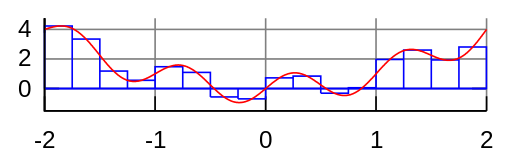
\includegraphics[width=\linewidth]{./gfx/03-rule01-rectangle}
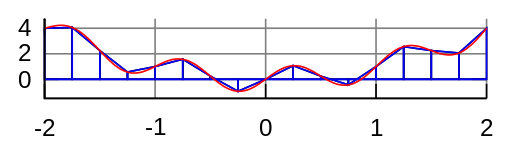
\includegraphics[width=\linewidth]{./gfx/03-rule02-trapezoid}
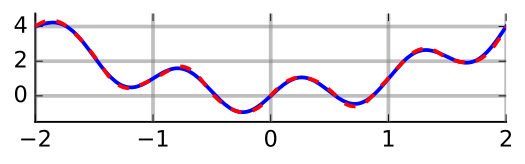
\includegraphics[width=\linewidth]{./gfx/03-rule03-simpson}
%
\emph{Computational Effort scales with order of polynomial, too.}
\end{minipage}
%
\end{frame}

% =========================================================================== %

\begin{frame}{Gaussian Quadrature}
%
\begin{itemize}
\item Idea: $\displaystyle \int_a^b f(x) \dd{x} \approx \sum_i^n w_i f(x_i)$
\item Get magic weights $w_i$ from assuming $f$ is a polynomial of degree $2n - 1$
\item Recursive formula for weights exists
\item Expensive to evaluate, for big $n$, but universally valid
\item[\Thus] Can be reused
\item[\Thus] Can be stored and re-loaded
\item Particular advantage: boundary values do not contribute to integral
	\begin{itemize}
	\item Useful in situations where derivatives are integrated
	\item Very high accuracy \emph{if well approximated by a polynomial}
	\end{itemize}
\item Requires internal rescaling
	\begin{itemize}
	\item Extra effort and chance for re-introducing rounding errors
	\end{itemize}
\end{itemize}
%
\end{frame}

% =========================================================================== %

\begin{frame}{Romberg Quadrature}
%
\begin{columns}
\column{.7\linewidth}
\begin{itemize}
\item \emph{Trapezoid rule on steroids}
\item Most time consuming part: evaluating $f(x)$
\item Compute initial estimate from $2^n + 1$ nodes via trapezoid rule
\item Half each interval by introducing new nodes
	\begin{itemize}
	\item Re-use known values for $f(x_i)$
	\item Get correction term for estimate of integral
	\item Iterate until correction term below some limit
	\end{itemize}
\item Very time-efficient due to adaptive number of evaluations
\item User-Friendly: provide accuracy parameter instead of number of nodes
\item Requires $2^{n+1}$ nodes -- not apt for all datasets
\end{itemize}
%
\column{.2\linewidth}
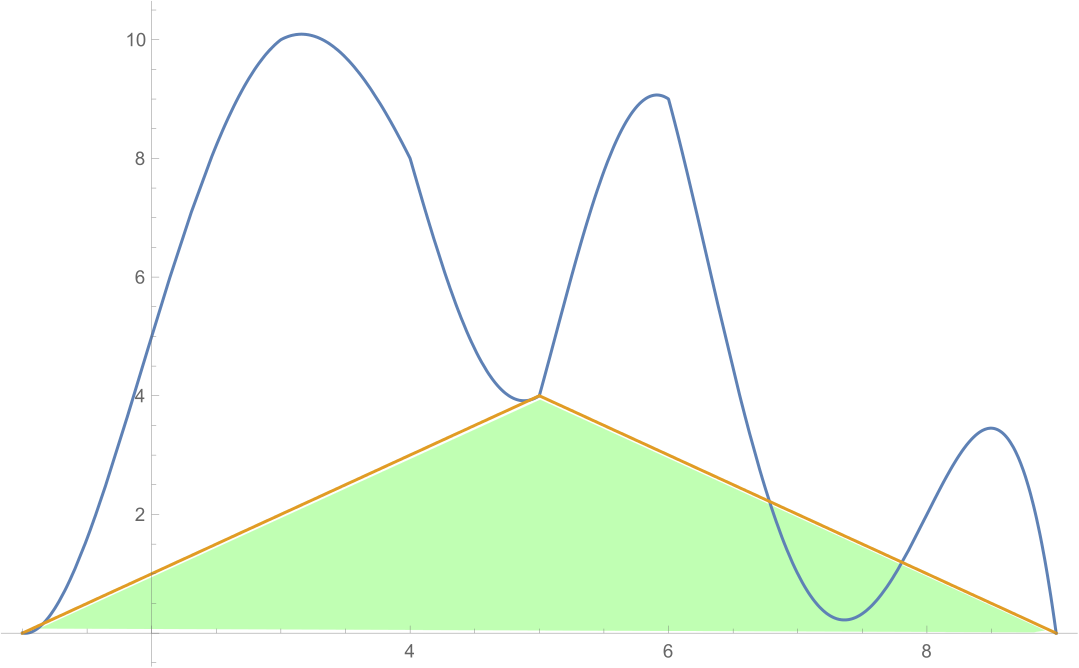
\includegraphics[width=\linewidth]{./gfx/03-romberg-01}
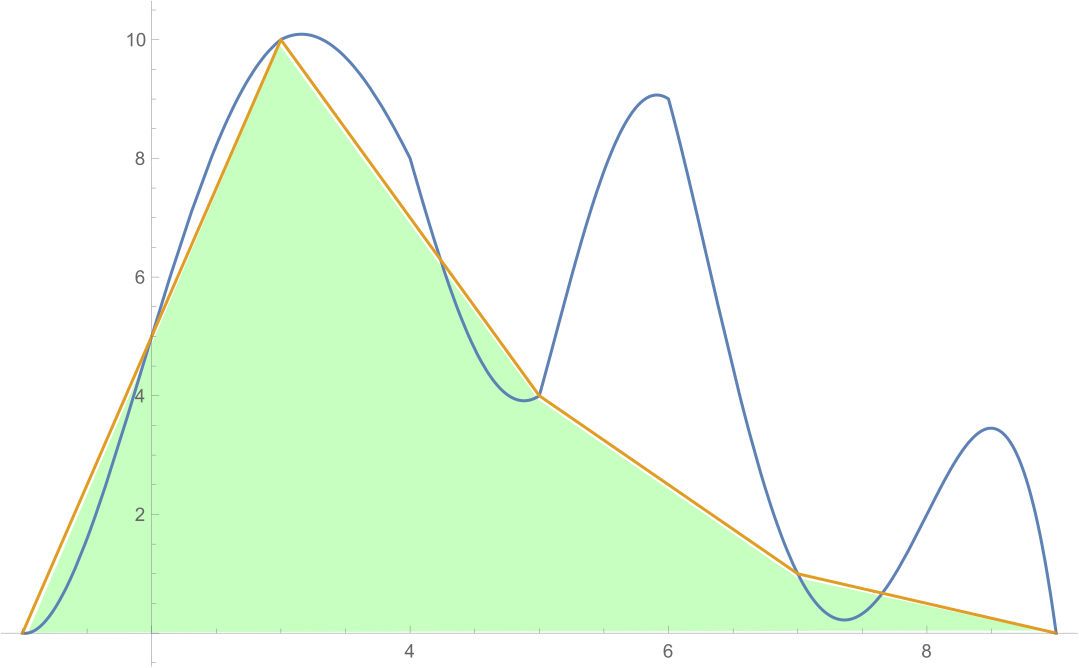
\includegraphics[width=\linewidth]{./gfx/03-romberg-02}
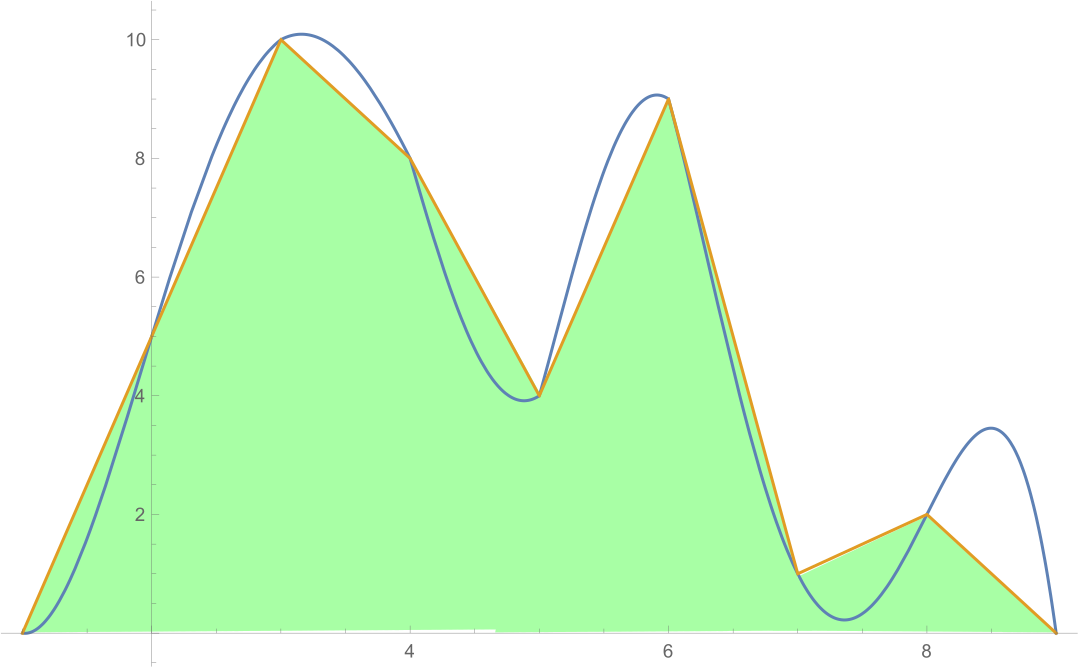
\includegraphics[width=\linewidth]{./gfx/03-romberg-03}
\end{columns}
%
\end{frame}

% =========================================================================== %

\begin{frame}{SciPy Implementations}
%
\begin{itemize}
\item All implementations in \texttt{scipy.integrate}
\item Implementations on a callable
	\begin{itemize}
	\item \texttt{quad} -- all purpose integral, highest accuracy, reasonable time requirements
	\item \texttt{quad\_vec} -- for vector valued functions
	\item \texttt{dblquad} and \texttt{tplquad} -- compute $\iint f(x, y) \dd{y}\dd{x}$ and $\iiint f(x, y, z) \dd{z}\dd{y}\dd{x}$
	\item \texttt{fixed\_quad} and \texttt{quadrature} -- Gaussian quadrature
	\item \texttt{romberg} -- Guess which quadrature
	\end{itemize}
\item Implementations on a pre-computed array
	\begin{itemize}
	\item \texttt{trapezoid}
	\item \texttt{simpson}
	\item \texttt{romb}
	\item Note: These work much faster, but require data to already be in memory
	\end{itemize}
\item For details, see \url{https://docs.scipy.org/doc/scipy/tutorial/integrate.html} 
\end{itemize}
%
\end{frame}

% =========================================================================== %

\begin{frame}
%
\begin{center}
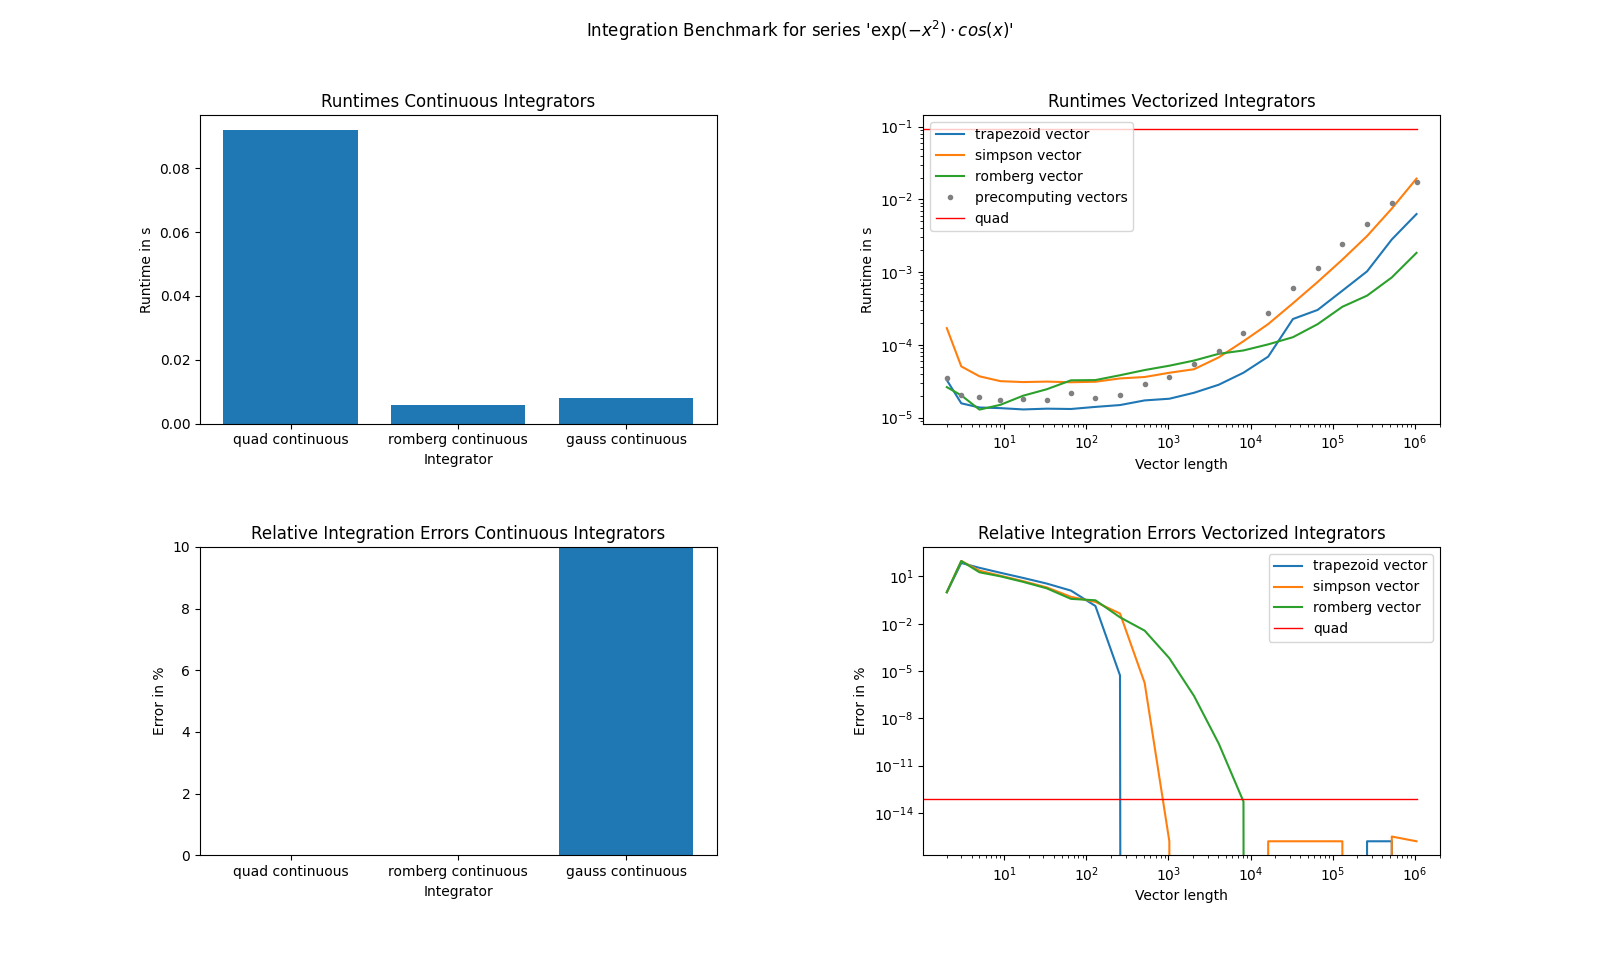
\includegraphics[width=\linewidth]{./gfx/03-timedints-1}
\end{center}
%
\end{frame}


% =========================================================================== %

\begin{frame}
%
\begin{center}
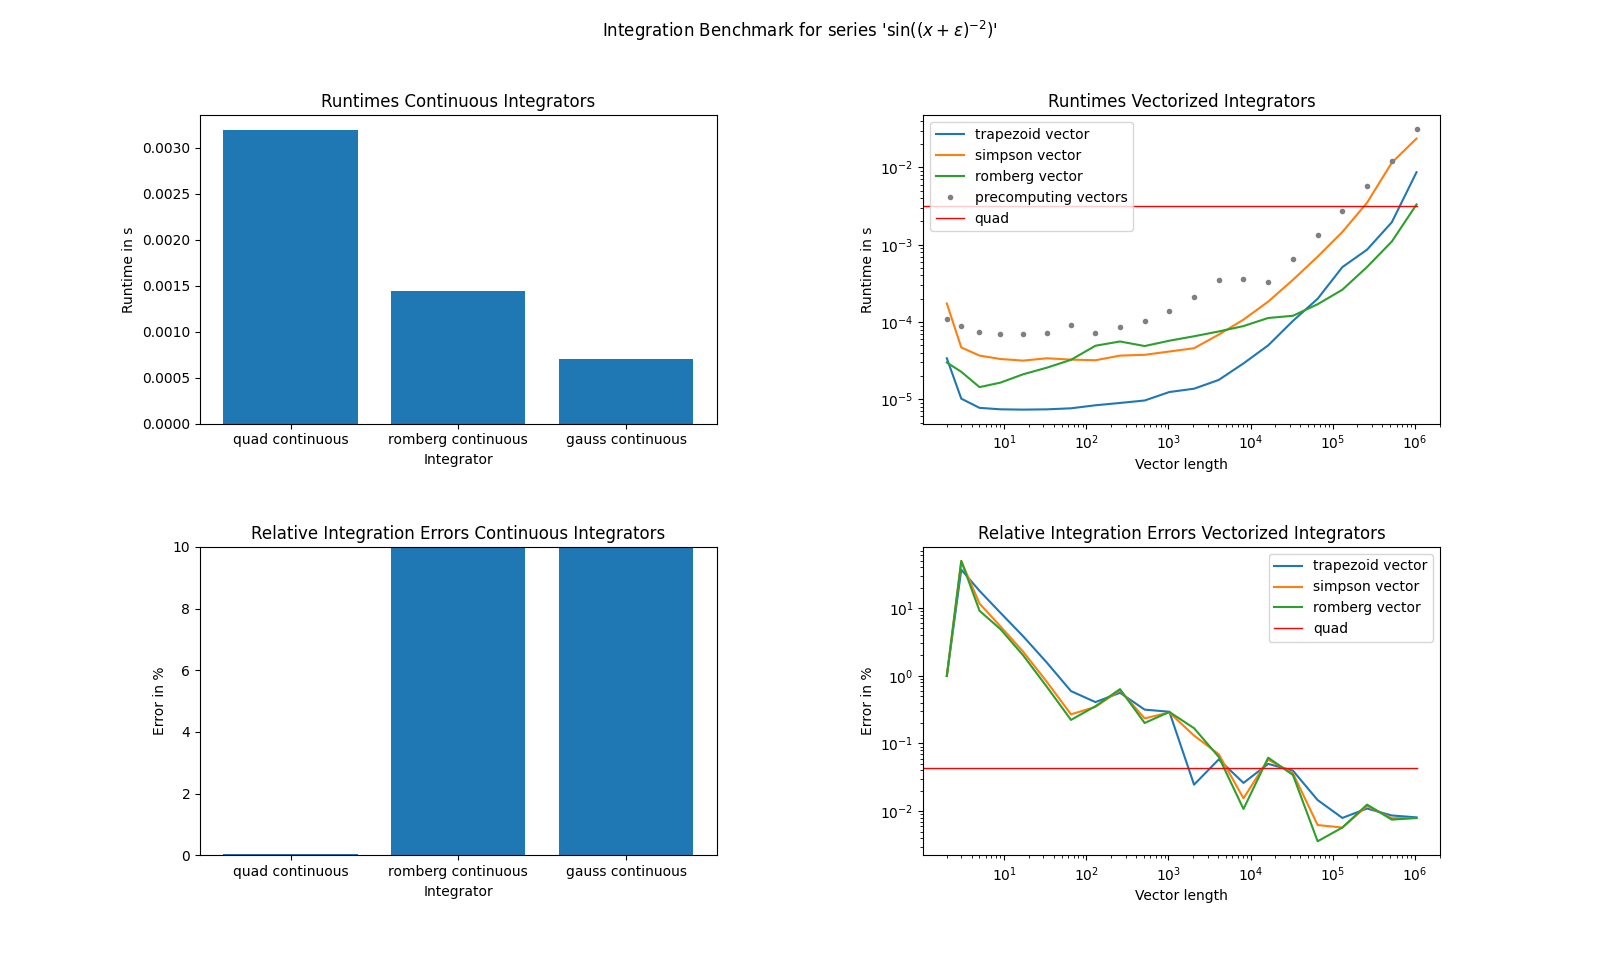
\includegraphics[width=\linewidth]{./gfx/03-timedints-2}
\end{center}
%
\end{frame}


% =========================================================================== %

\begin{frame}
%
\begin{center}
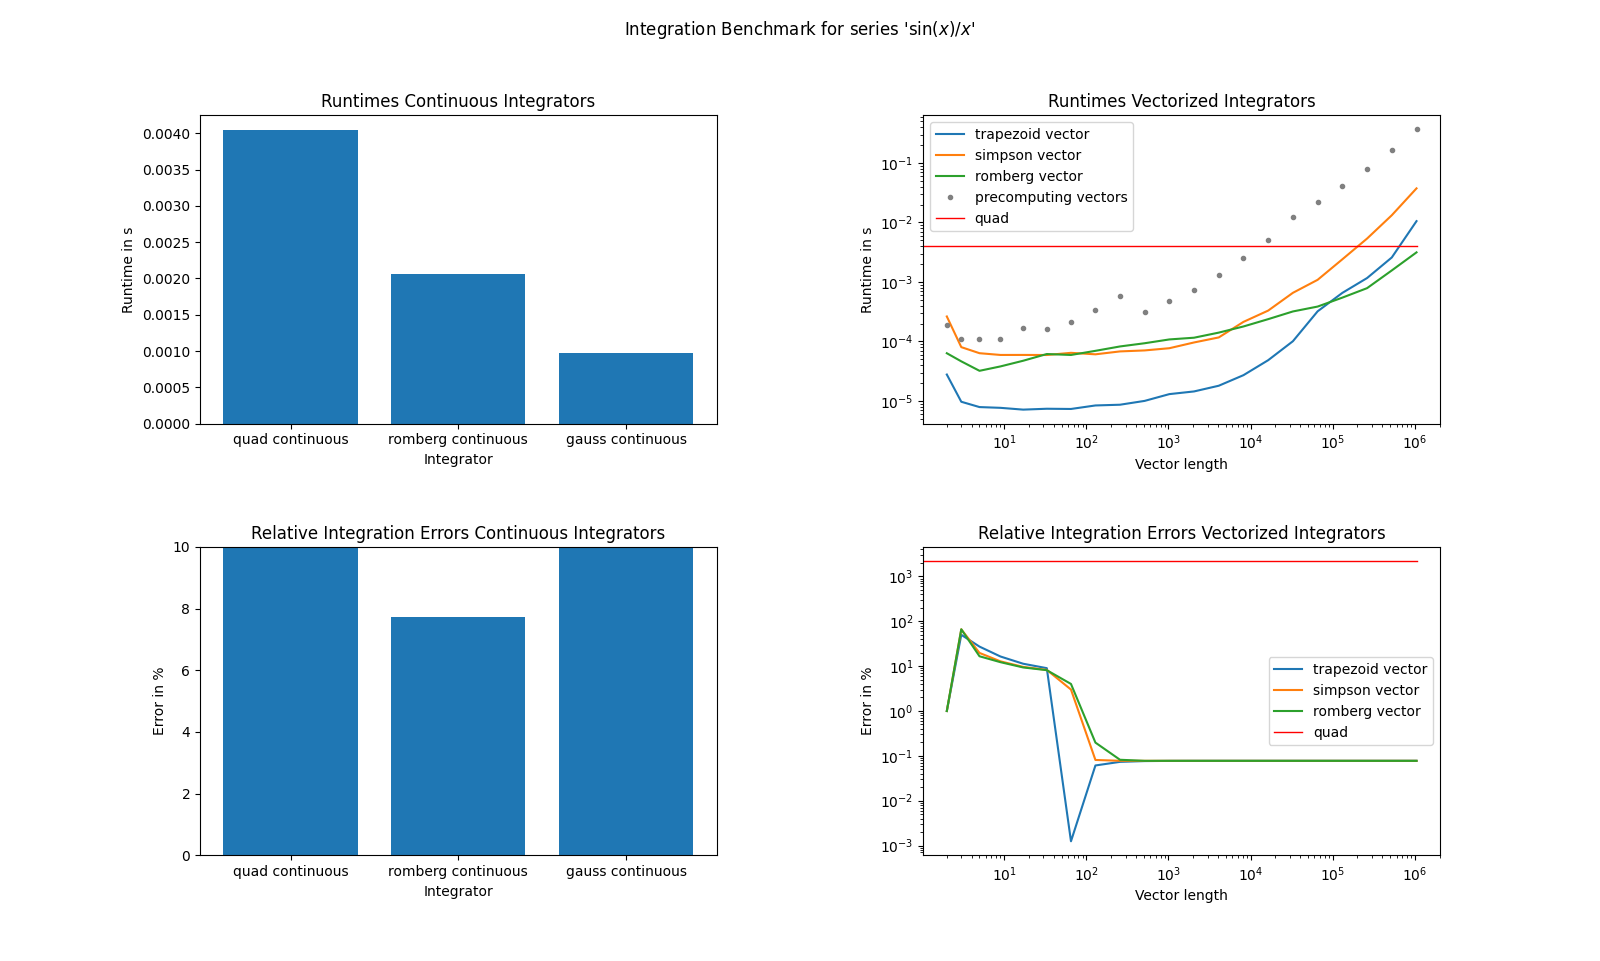
\includegraphics[width=\linewidth]{./gfx/03-timedints-3}
\end{center}
%
\end{frame}

% =========================================================================== %

\begin{frame}[fragile]{Beware of Periodic Functions When Using Romberg}
%
\begin{codebox}[Romberg Fails Periodic Functions]
\begin{minted}[linenos, fontsize=\scriptsize]{python3}
f = lambda x: np.abs(np.sin(x))
n = 10
X = np.linspace(0, 2 * np.pi, 2 ** n + 1)
Y = f(X)

I = scipy.integrate.quad(f, X[0], X[-1])
R = scipy.integrate.romberg(f, X[0], X[-1])

print(f"Generic integration yielded {I[0]} +/- {I[1]}")
print(f"Romberg integration yielded {R}.")
\end{minted}
\end{codebox}
%
\begin{cmdbox}[Output: Romberg Fails Periodic Functions]
\begin{minted}[fontsize=\scriptsize]{text}
Generic integration yielded 4.0 +/- 4.440892098500626e-14
Romberg integration yielded 7.694682774887159e-16.
\end{minted}
\end{cmdbox}
%
\end{frame}

% =========================================================================== %\\

\begin{frame}{Take-Aways}
%
\begin{itemize}
\item \texttt{quad} does a very good job most of the time, but is relatively slow
\item Vector-Based integrators require extra-time for computing the vector, but can beat \texttt{quad} in both, time and accuracy
	\begin{itemize}
	\item Trapezoid fastest
	\item Simpson slightly more accurate, often little difference
	\end{itemize}
\item Other function-based integrators can do better than both, but are error-prone
\item Gaussian quadrature works very badly when integrand not well approximated by a polynomial
	\begin{itemize}
	\item This also holds for \emph{infinite} polynomials such as \texttt{exp}, \texttt{sin}
	\item And for \emph{negative powers} like $\dfrac{1}{x}$ etc
	\end{itemize}
\item Romberg bad when dealing with periodic functions
\end{itemize}
%
\end{frame}

\end{document}

% MAREI!!
% whom do I give credit? Where?